\chapter{Modelagem e Simulação} \label{cap3}

Neste capítulo será descrito a modelagem do sistema, o processo de estimação de velocidade do vento, e a simulação do túnel de vento no Simulink Matlab.

\section{Descrição da Planta}
O sistema em questão se trata de um tubo PVC de 40 mm de 120 cm, ele é afixado em uma plataforma plástica através de uma base e de elásticos para estabilização. Na ponta inferior do tubo se encontra uma turbina de avião RC que empurra o ar para dentro do tubo elevando uma bola de tênis de mesa, na ponta superior do tubo se encontra um sensor infravermelho de distância. A turbina é controlado por um Arduino Mega 2560.

\section{Modelo Matemático}



\commentib{inserir figura do sistema}\label{fig:sistemasimples}

Há duas forças atuantes na esfera, a gravidade que a puxa para baixo e a força de empuxo gerada pelo vento. Obtemos a seguinte equação do movimento:
\begin{equation}
m \ddot{h}=F=\dfrac{1}{2} \cdot C_a \cdot\rho \cdot A \cdot (v_a- \dot{h})^2-m\cdot g
\end{equation}

onde $m$ é a massa da esfera, $h$ é a posição vertical da esfera no tubo, $\rho$ é a densidade do ar, $A$ é a área da esfera em contato com o fluxo de ar, $v_a$ é a velocidade do ar dentro do tubo e $C_a$ é o coeficiente aerodinâmico da esfera. O coeficiente aerodinâmico depende da velocidade relativa entre a esfera e o vento, mas para as velocidades baixas de vento que estamos utilizando esse valor pode ser considerado constante. Consideramos $\alpha= \dfrac{1}{2} \cdot C_a \cdot \rho \cdot A$:
\begin{equation} \label{eq:modelo}
\ddot{h}=\dfrac{\alpha}{m}\cdot (v_a-\dot{h})^2-g
\end{equation}

\section{Estimação da Velocidade do Vento}
Para criarmos um simulador do sistema descrito anteriormente precisamos saber o valor de $v_a$. Ele determina a velocidade do vento para diferentes valores de tensão e altura da bola. Não foi possível adquirir um sensor de velocidade do ar devido a problemas de localização geológica, portanto, foi necessário usar de engenhosidade para adquirir a velocidade do ar em diversas alturas.


Foram adquiridas diversas bolas de tênis de mesa e se injetou uma mistura de cola e água nelas para aumentar o seu peso. Foram escolhidos 6 pesos diferentes e medidos em balança com precisão de duas casas decimais. Então para cada peso foi medida a tensão necessária para que se alcance as 6 alturas dentro da região de funcionamento do sensor, 10, 20, 30, 40, 50, 60 cm. Tendo medido a altura e a tensão necessária para alcançar as alturas, bastou utilizar a equação \ref{eq:modelo} fazendo $\ddot{h}=\dot(h)=0$ para obter a velocidade do vento relacionada com uma altura e uma tensão.

\begin{figure}[h]
	\centering
	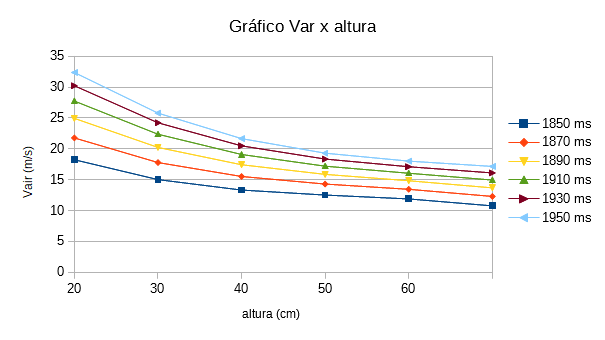
\includegraphics{grafico_vair_altura}
	\caption[Gráfico $v_a$ x altura]{Gráfico de $v_a$ x altura}
	\label{fig:graficovairaltura1}
\end{figure}

Podemos ver que a figura \ref{fig:graficovairaltura1} lembra um gráfico similar encontrado em \cite{jernigan2009} onde o autor utiliza um sensor de velocidade de vento e mostra uma curva similar, para uma mesma tensão aplicada na turbina quanto mais elevada se encontra a bola menor vai ser a velocidade do ar que se choca com ela.

\section{Simulação do Túnel de Vento no Simulink}

Criamos um modelo de simulação à partir da equação \ref{eq:modelo} e utilizamos os dados adquiridos em \ref{fig:graficovairaltura1} para fazer um ajuste de curva que alimenta o modelo com os valores da velocidade do vento para determinada altura e tensão no motor.

\begin{figure}[h]
	\centering
	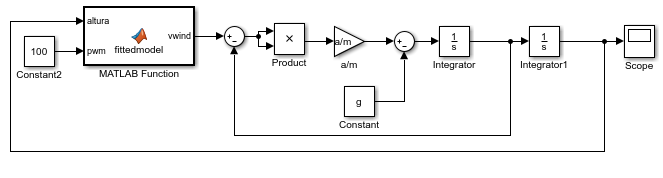
\includegraphics{simulador}
	\caption[Simulador do túnel de vento]{Simulador do túnel de vento}
	\label{fig:simulador}
\end{figure}




% Fim Capítulo
